% ###################################################
% Title:			  Current resume
% Author:			  bmarron
% Origin Date:	22 Mar 2017	
% Final Date:	  
%
%
% ############################################################
% %%%%%%%%%%%%%%%%%%%%%%%%%%%%%%%%%%%%%%%%%%%%%%%%%%%%%%%%%%%%
% You can have multiple style options the legal options ones are:
%
%   centered	
%   the name and address are centered at the top of the
%		page (default)
%
%   line	
%   the name is the left with a horizontal line then 
%		the address to the right
%
%   overlapped	
%   the section titles overlap the body text (default)
%
%   margin	
%   the section titles are to the left of the body text
%		
%   11pt	
%   use 11 point fonts instead of 10 point fonts
%
%   12pt	
%   use 12 point fonts instead of 10 point fonts
%
%%%%%%%%%%%%%%%%%%%%%%%%%%%%%%%%%%%%%%%%%%%%%%%%%%%%%%%%%%%%%
%%%%%%%%%%%%%%%%%%%%%%%%%%%%%%%%%%%%%%%%%%%%%%%%%%%%%%%%%%%%%
%  Commands (available in res.cls)
%%%%%%%%%%%%%%%%%%%%%%%%%%%%%%%%%%%%%%%%%%%%%%%%%%%%%%%%%%%%%
% \Resume
% prints the word resume but typeset nicely
%
%\newsectionwidth{dimen}
%		defines the amount of space the labels extend
%		into the left margin.
%		DO NOT TRY to change any of the dimensions
%		yourself.  You will probably confuse the style file.
%
%\name{text} 
% defines your name
%
% \address{text}
%		defines your address
%		this can be called twice if you have two addresses
%		use \\'s to indicate where either line breaks or
%		comas should go
%
% \opening	
%   this prints your name and address at that spot
%		this is not normally needed, as \begin{resume}
%		does this but is provided just in case you need
%		to do something odd
%
% \begin{resume} ... \end{resume}
%		all of the resume should go inside of this
%		environment
%
% \section{text}
%		This prints 'text' in the left hand margin.
%		Its exact placement depends on what the style 
%		options has been set to. (overlapped or margin)
%		You should use \\ to start a new line.	If the
%		style option is margin, the \\ is converted
%		to a space.	To use this in any of the list environments, put
%		the \section after the \item[] but before the 
%		text.
%		Eg.
%		\begin{itemize}
%		\item\section{text}
%		text
%		\end{itemize}
%
% \begin{ncolumn}{n} ... \end{ncolumn}
%		creates a tabular environment with n equally
%		spaced columns.  Separate columns by & and
%		end them with \\
%
% \begin{position} ... \end{position}
%		this is used to print a job description.  There should
%		be only one job description in it.  Information
%		related to the job (such as title, dates...) will
%		be printed.
%
%  eg.
%\section{EXPERIENCE}
%\employer{Employer One}
%\location{Location One}
%\dates{Dates One}
%\title{\textbf{Title One}}
%\begin{position}
%Vivamus ullamcorper a lacus non laoreet. Etiam ultricies in est quis finibus. 
%Curabitur posuere est quis felis sodales, vitae aliquam ex consequat. In non 
%magna felis.
%\end{position}
%
%
% \begin{format} ... \end{format}
%		used to change the default format for the position
%		environment.  Within it the recognized commands are:
%		\title{option}
%		\employer{option}
%		\location{option}
%		\dates{option}
%		\body
%		\\
%		where option is one of l,r,c standing for left, right, center.
%		The format will eventually be used to make several
%		tabular environments and you are defining the number of columns
%		and the placement of text within the columns of the tabulars.
%		Each row is terminated by a \\.  Any number of options can 
%		be on a line, they will each be set in their own columns.
%		Any of the options except \body may be left out.
%
%		Eg.
%		\begin{format}
%		\title{l}\employer{r}\\
%		\dates{r}\\
%		\body\\
%		\location{l}\\
%		\end{format}
%
%		In this example the title and employer information
%		are set in 2 columns left justified and right justified
%		respectively.  Then the date is set right justified.
%		Then the body is set.  Then the location is set left
%		justified.
%
% \employer{text}
% \title{text}
% \dates{text}
% \location{text}
%		declare text for the next invocation of the position
%		environment
%%%%%%%%%%%%%%%%%%%%%%%%%%%%%%%%%%%%%%%%%%%%%%%%%%%%%%%%%%%%%%%%%%%%%%


\documentclass[line]{res}
\resumewidth=7.5in

\usepackage[scale=0.93]{geometry}
%\usepackage[left=0.5in, right=0.5in, top=0.5in, bottom=0.5in]{geometry}
\usepackage{wrapfig}
\usepackage{csquotes}
\usepackage{newcent}

\usepackage{fancyhdr} % Headers and footers
%\pagestyle{fancy} % All pages have headers and footers
%\fancyhead[L]{\date{\today}}
%\fancyfoot[R]{\thepage} % Custom footer text

\usepackage{graphics}
\usepackage{tikz}  
%\renewcommand\labelitemi{{\boldmath$\cdot$}}  %medium bullets


% ###########
% DOCUMENT
% ###########
\newsectionwidth{0.5cm}

\begin{document}

\name{Bruce D. Marron}
\address{Vito Alessio Robles 237, CDMX, CP 01050}
\address{Contact: marron.bruce.mx@gmail.com; +52 55 4190 9628}

 
\begin{resume}

%%%%%%%%%%%%%%%%%%%%
\section{Identity}
%%%%%%%%%%%%%%%%%%%%%
\textbf{NUE:} 2172716 (Residente Permanente) \\
\textbf{Passport:} A36267253 (USA, exp. 14 Mar 2034) \\
\textbf{RFC:} MABR5903193S6 \\
\textbf{CURP:} MAXB590319HNERXR03


%%%%%%%%%%%%%%%%%%%%
\section{Fine Arts Education}
%%%%%%%%%%%%%%%%%%%%%
\textbf{Music studies}, Portland State University, 1999-2000 \\
\textbf{Music studies}, University of New Mexico, 1996-1997 \\
(36 hours in music theory, ear training, basic piano, music history, applied music, jazz band, jazz imrpovisation) \\
\textbf{Private Lessons}, Classical guitar with Michael Chapdelaine, classical and fingerstyle master 1996-1997 \\
\textbf{Private Lessons}, Jazz guitar with Michael Anthony, LA studio guitarist 1994-1997


%%%%%%%%%%%%%%%%%%%%
\section{Science Education}
%%%%%%%%%%%%%%%%%%%%%
\textbf{Doctoral studies}, Portland State Univ. (PSU) and North Carolina State Univ. (NCSU), 2015-2017\\
\textbf {Graduate Certificate in Statistics}, PSU, 2017 \\
\textbf{M.S., Systems Science}, PSU, 2015 \\
\textbf {Graduate Certificate in Sustainability}, PSU, 2012 \\
\textbf{M.S., Chemistry}, New Mexico Tech, 1989 \\
\textbf{B. Sci. Ed.}, University of New Mexico, 1985


%%%%%%%%%%%%%%%%%%%%%%
\section{Academic Awards}
%%%%%%%%%%%%%%%%%%%%%%%
\begin{itemize}
\itemsep -2pt % reduce space between items
\item National Science Foundation ESUR-IGERT Fellowship, Portland State University
\item Presidential Scholarship, University of New Mexico
\end{itemize}


%%%%%%%%%%%%%%%%%%%%
\section{Human Languages}
%%%%%%%%%%%%%%%%%%%%%
English (Native) \\
Spanish (B2/C1)

%%%%%%%%%%%%%%%%%%%%%%%%%%
\section {Relevant Teaching Experience}
%%%%%%%%%%%%%%%%%%%%%%%%%
{\sl Universidad Tecnología de America (UTECA), CDMX, México} \hfill Jan 2025 - present \\
(Melissa Verduzco Villarruel, Rector) \\
Contracted for the development and classroom delivery of specialized, college-level curriculum in the areas of science and technology, law, economics, and advanced English that fulfill requirements for the Bachelor's degree in Translation and Interpretation (\textit{Licenciatura en Traducción y Interpretación}). In all classes, a constructivist approach to learning is used with an emphasis on basic skills: reading, writing, and speaking. Key components of the curriculum include: i) reading, analysis, discussion, and written critique of award-winning English language novels; ii) analysis and review of topical investigations in science, technology, civil law, international law, economics, records management, professional consulting, and the professional use of artifical intelligence (AI); and iii) grammatical supplements from Raymond Murphy's, \textit{English Language in Use (5th ed.)} and Strunk and White's, \textit{Elements of Style}.

{\sl Avalon International School, CDMX, México} \hfill Jan 2024 - Dec 2024 \\
(Gonzalo Alejandro Esteva Luna Parra, Director) \\
English language arts teacher and curriculum development specialist for 5th grade, 8th grade, and 9th grade ESL students. Taught under the auspices of the International Baccalaureate (IB) Program for 5th grade, and developed a specialized curriculum for 8th and 9th grade students. The middle school Second Language Acquisition (SLA) curriculum coupled a comptence driven, communicative approach with a task-based teaching style. 

{\sl Catholic Charities, Portland, Oregon} \hfill 2015 \\
(Vilma Chan Vasquez, School Based Services Program Manager) \\
Teacher and curriculum development specialist for {\sl Puentes}, an eight-week, summer mathematics program for Latino youth. The Puentes program provided a structured but home-like environment for kids needing extra help in English and mathematics. Much of the interaction and instruction was in Spanish. 

\vspace{0.9cm}

{\sl Portland Public School, Portland, Oregon} \hfill 2000-2010\\
(Toni Hunter, Grant HS;  Peg Lewis, Kellogg MS)\\
Teacher (chemistry, foundations of physics and chemistry, forensic science (HS); math, science and health (MS)) and curriculum development specialist; author of HS curriculum entitled, \enquote{Sustainability: Transitioning to Adaptive Resilience in a Post-Carbon World}; author of spreadsheet-based, qualitative analysis curriculum; logistics manager of chemistry lab equipment and supplies; recruitment and management of student and parent volunteers. First aid, CPR, and AED trained.

{\sl Starfire Music, Albuquerque, New Mexico} \hfill 1996-1998\\
(Bruce Marron, Owner)\\
Guitar and music instructor to adults and kids.

%%%%%%%%%%%%%%%%%%%%%%%%%%
\section {Relavant Fine Arts Experience}
%%%%%%%%%%%%%%%%%%%%%%%%%

{\sl MOZ, Ciudad de Mexico, Mexico} \hfill 2023\\
Fundador del colectivo MOZ, productor y musico para el espectaculo, \enquote{CONTINENTAL Pop Rock Theater}.  El función fue una exploración de música rock y pop mezclado con teatro y performance art. Presentando composiciones musicales completamente originales y algunos covers.  Presentando también obras originales de teatro y performance art. Se llevó a cabo en el {\sl Foro Cultural Coyoacanense Hugo Argüelles}, el día 26 de agosto 2023.

{\sl La Marconi, Ciudad de Mexico, Mexico} \hfill 2023\\
Guitarista de jazz y pop para shows de La Marconi (cantante) en Hermes Music Club (Centro Histórico) y Ciao Mamma Restaurante (Interlomas).

{\sl Lucky vs The Bomb, Portland, Oregon} \hfill 2001-2005\\
Singer-songwriter and performer for the indie rock band {\sl Lucky vs The Bomb}.

{\sl Missoula Children's Theater, Missoula, Montana} \hfill 1999\\
Orquestral guitarist for the musical production of \textit{Fiddler on the Roof}. 

{\sl Albuquerque Civic Light Opera, Albuquerque, New Mexico} \hfill 1996-1998\\
Orquestral guitarist for the musical productions of \textit{Godspell, Sound of Music, and Camelot}. 


%% Pic 1
\begin{tikzpicture}[overlay]
  \node[anchor=south west] at (0.4,-5.5) {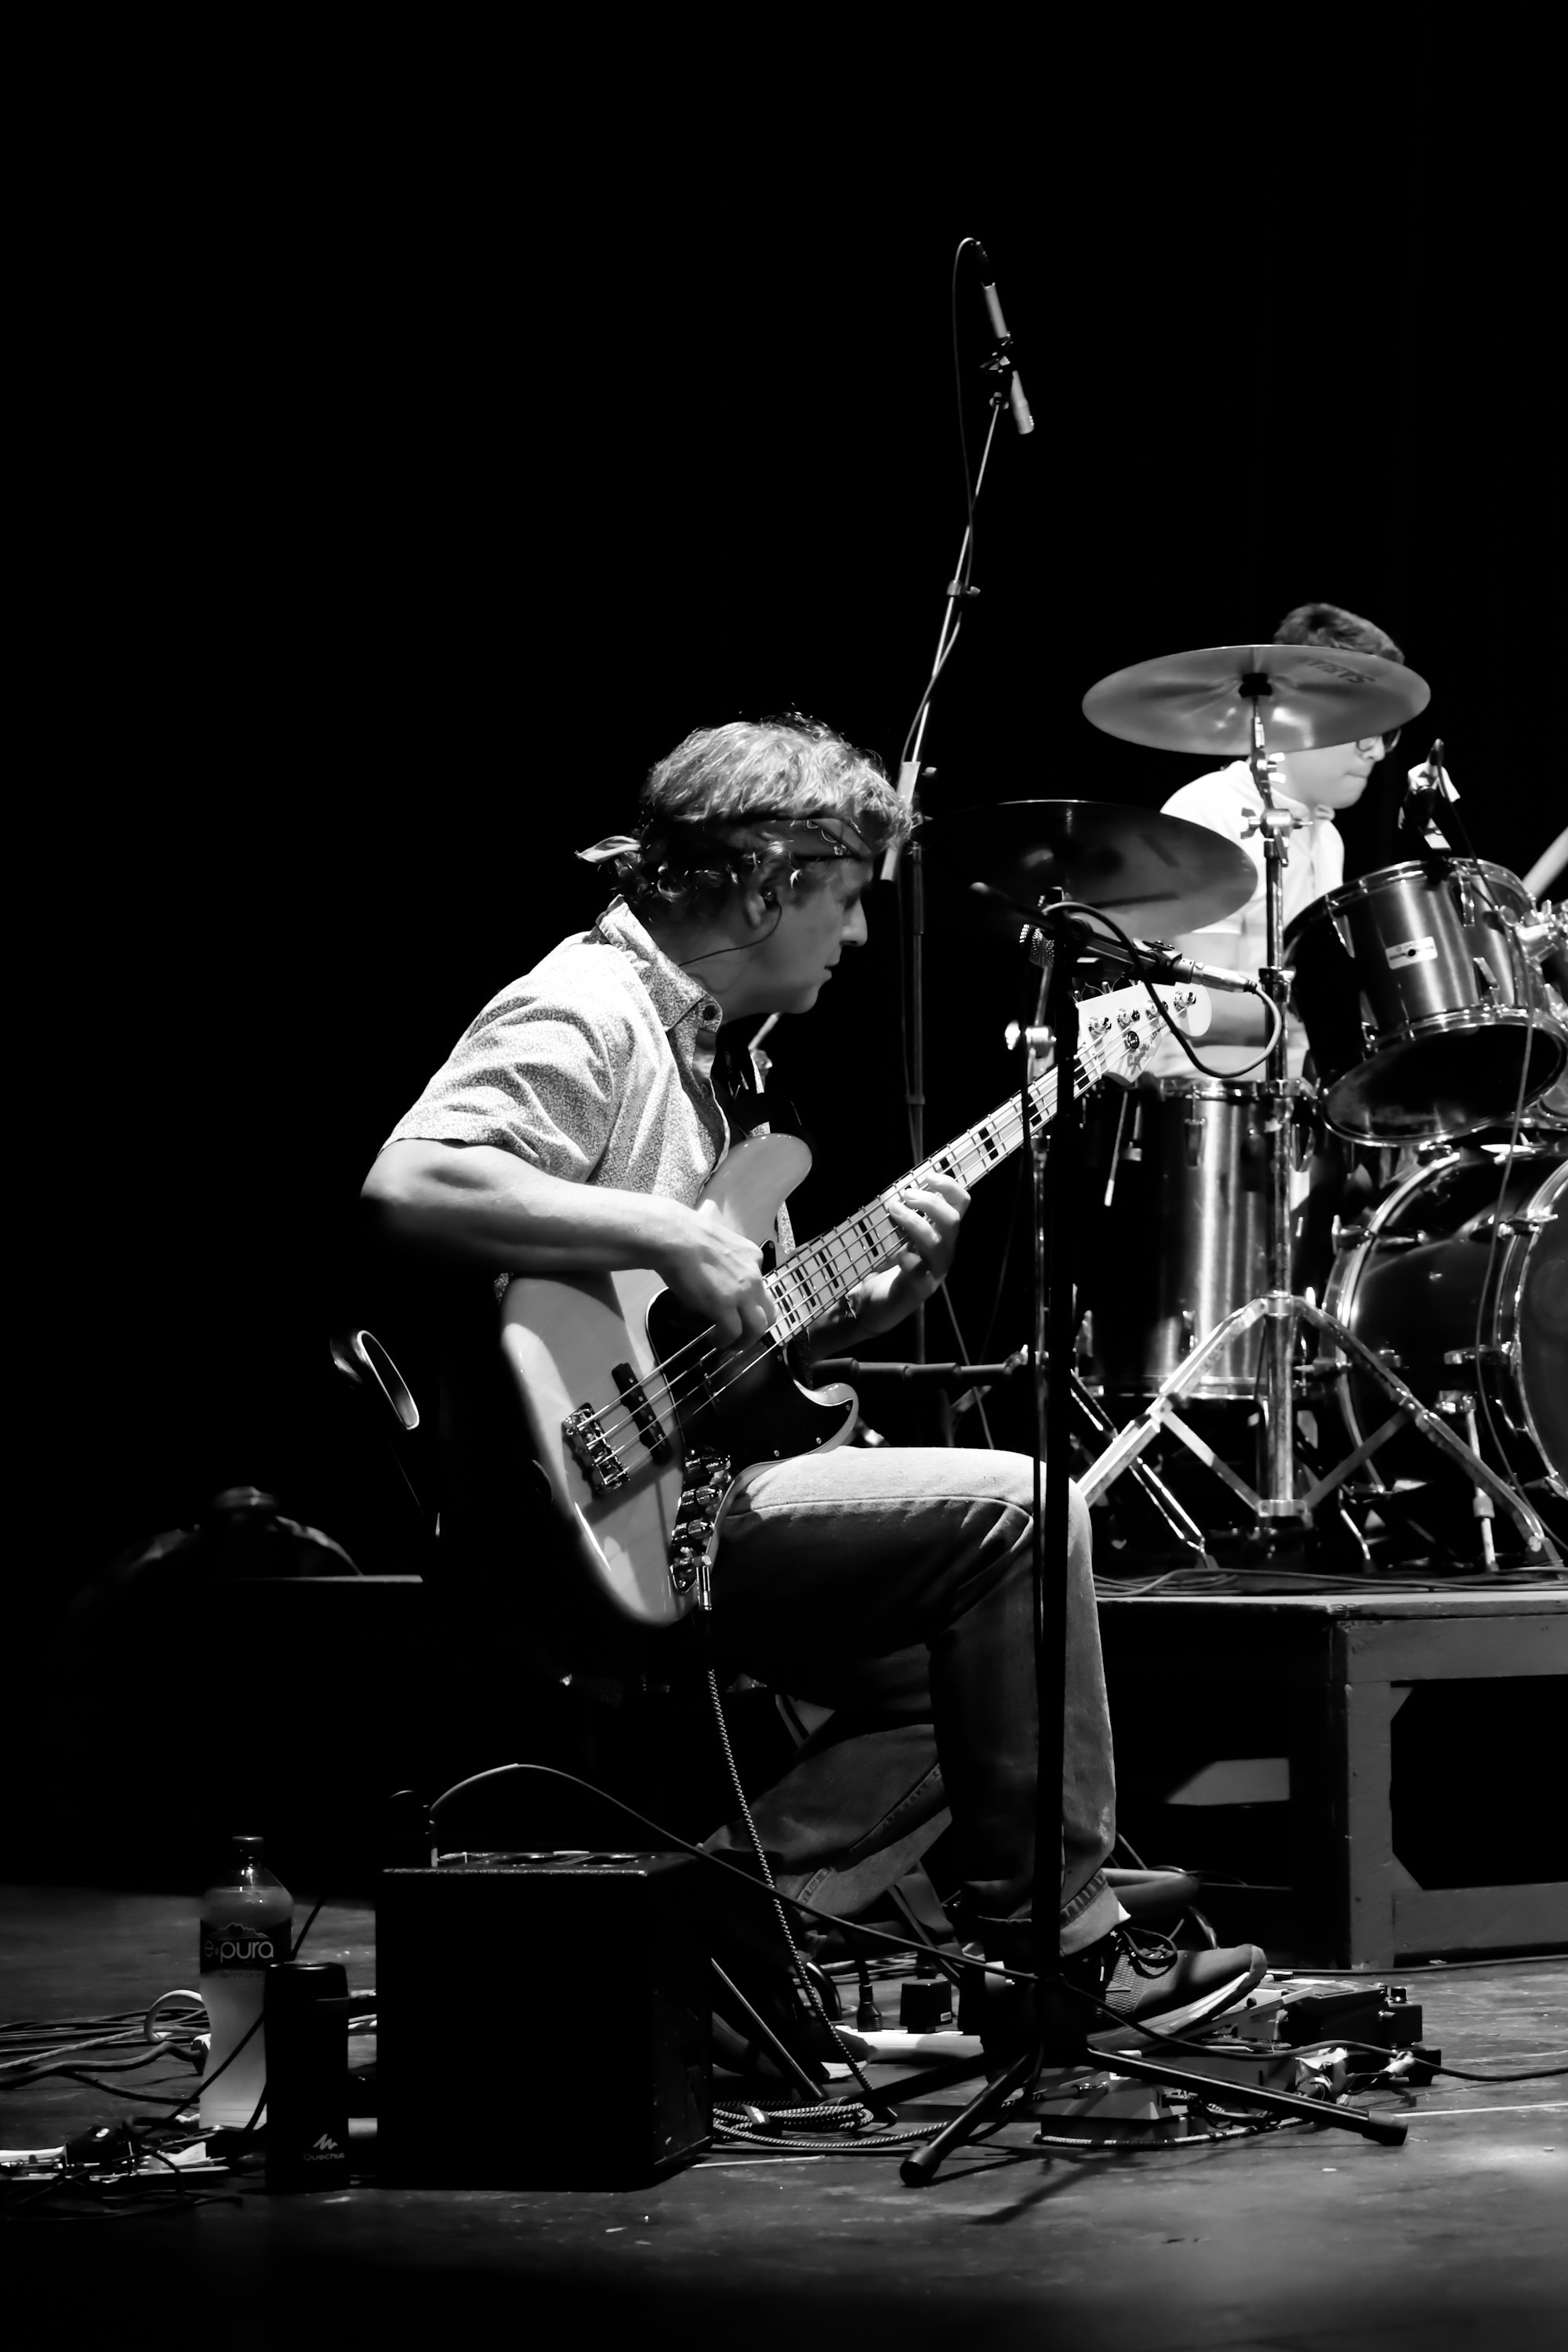
\includegraphics[scale=0.05]{graphics/Marron_Bass.jpeg}};  
 \end{tikzpicture}
 
 %% Pic 2
 \begin{tikzpicture}[overlay]
  \node[anchor=south west] at (7,-5.0) {\includegraphics[scale=0.11]{graphics/Marron_Photoshoot.png}};  
 \end{tikzpicture}
 
 %% Pic 3
 \begin{tikzpicture}[overlay]
  \node[anchor=south west] at (13,-4.8) {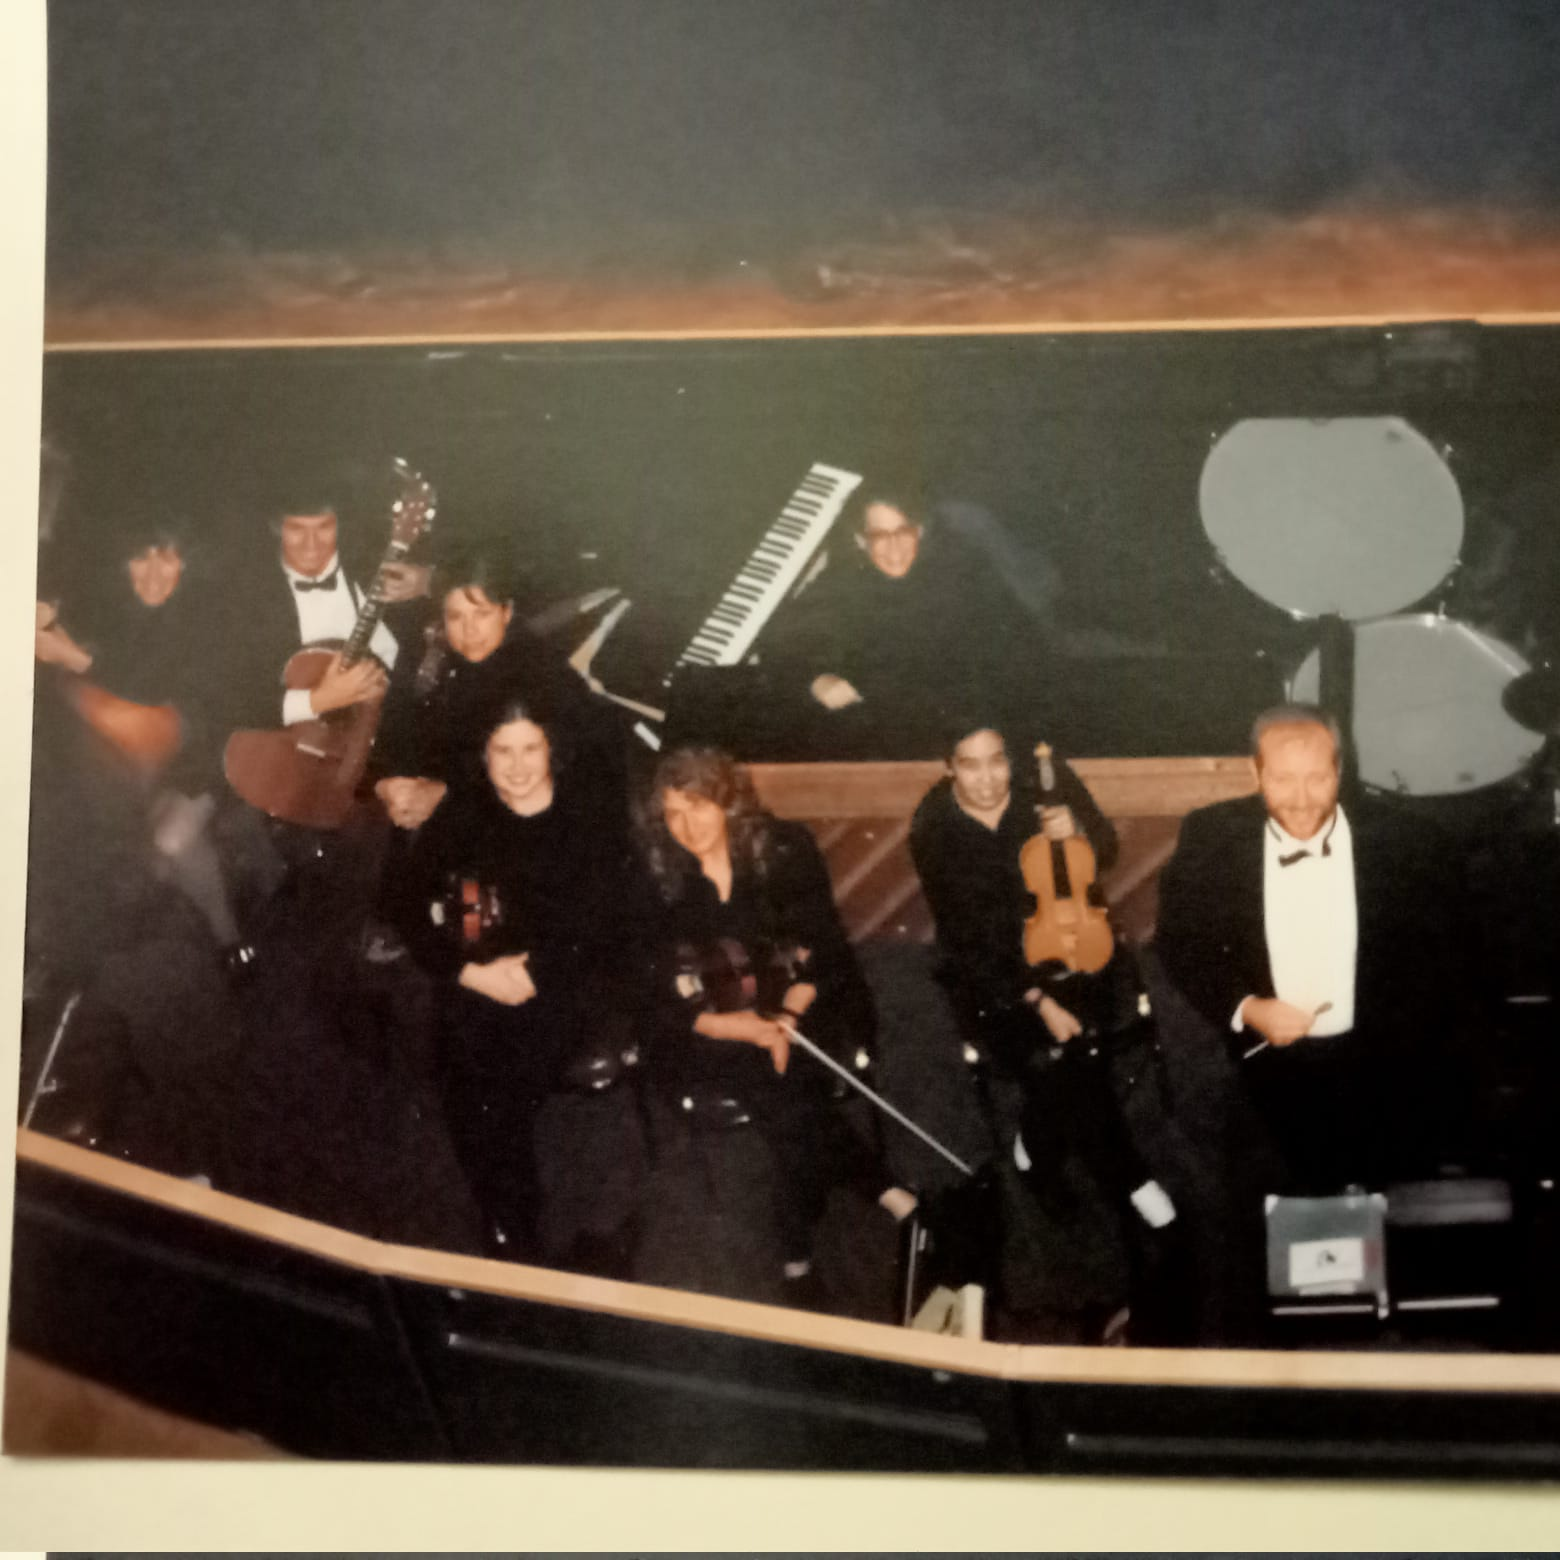
\includegraphics[scale=0.11]{graphics/Marron_Orchestra.jpeg}};  
 \end{tikzpicture}
 
 %% Pic 4
 \begin{tikzpicture}[overlay]
  \node[anchor=south west] at (0.1,-7.5) {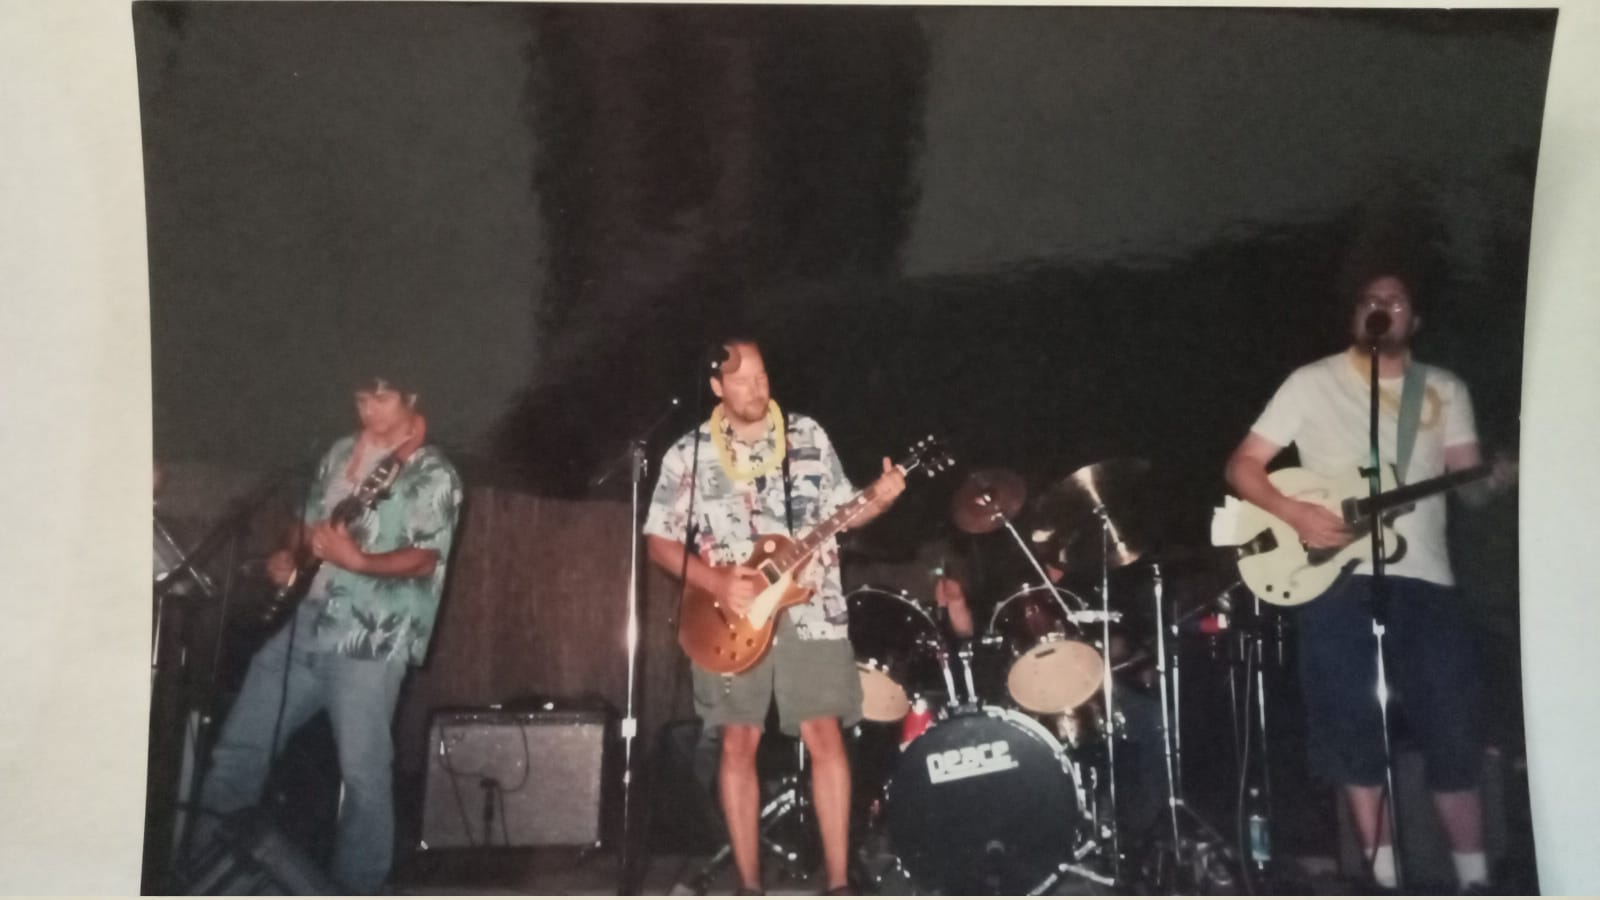
\includegraphics[scale=0.1]{graphics/Marron_LVTB.jpeg}};  
 \end{tikzpicture}
 
  %% Pic 5
 \begin{tikzpicture}[overlay]
  \node[anchor=south west] at (7,-9.0) {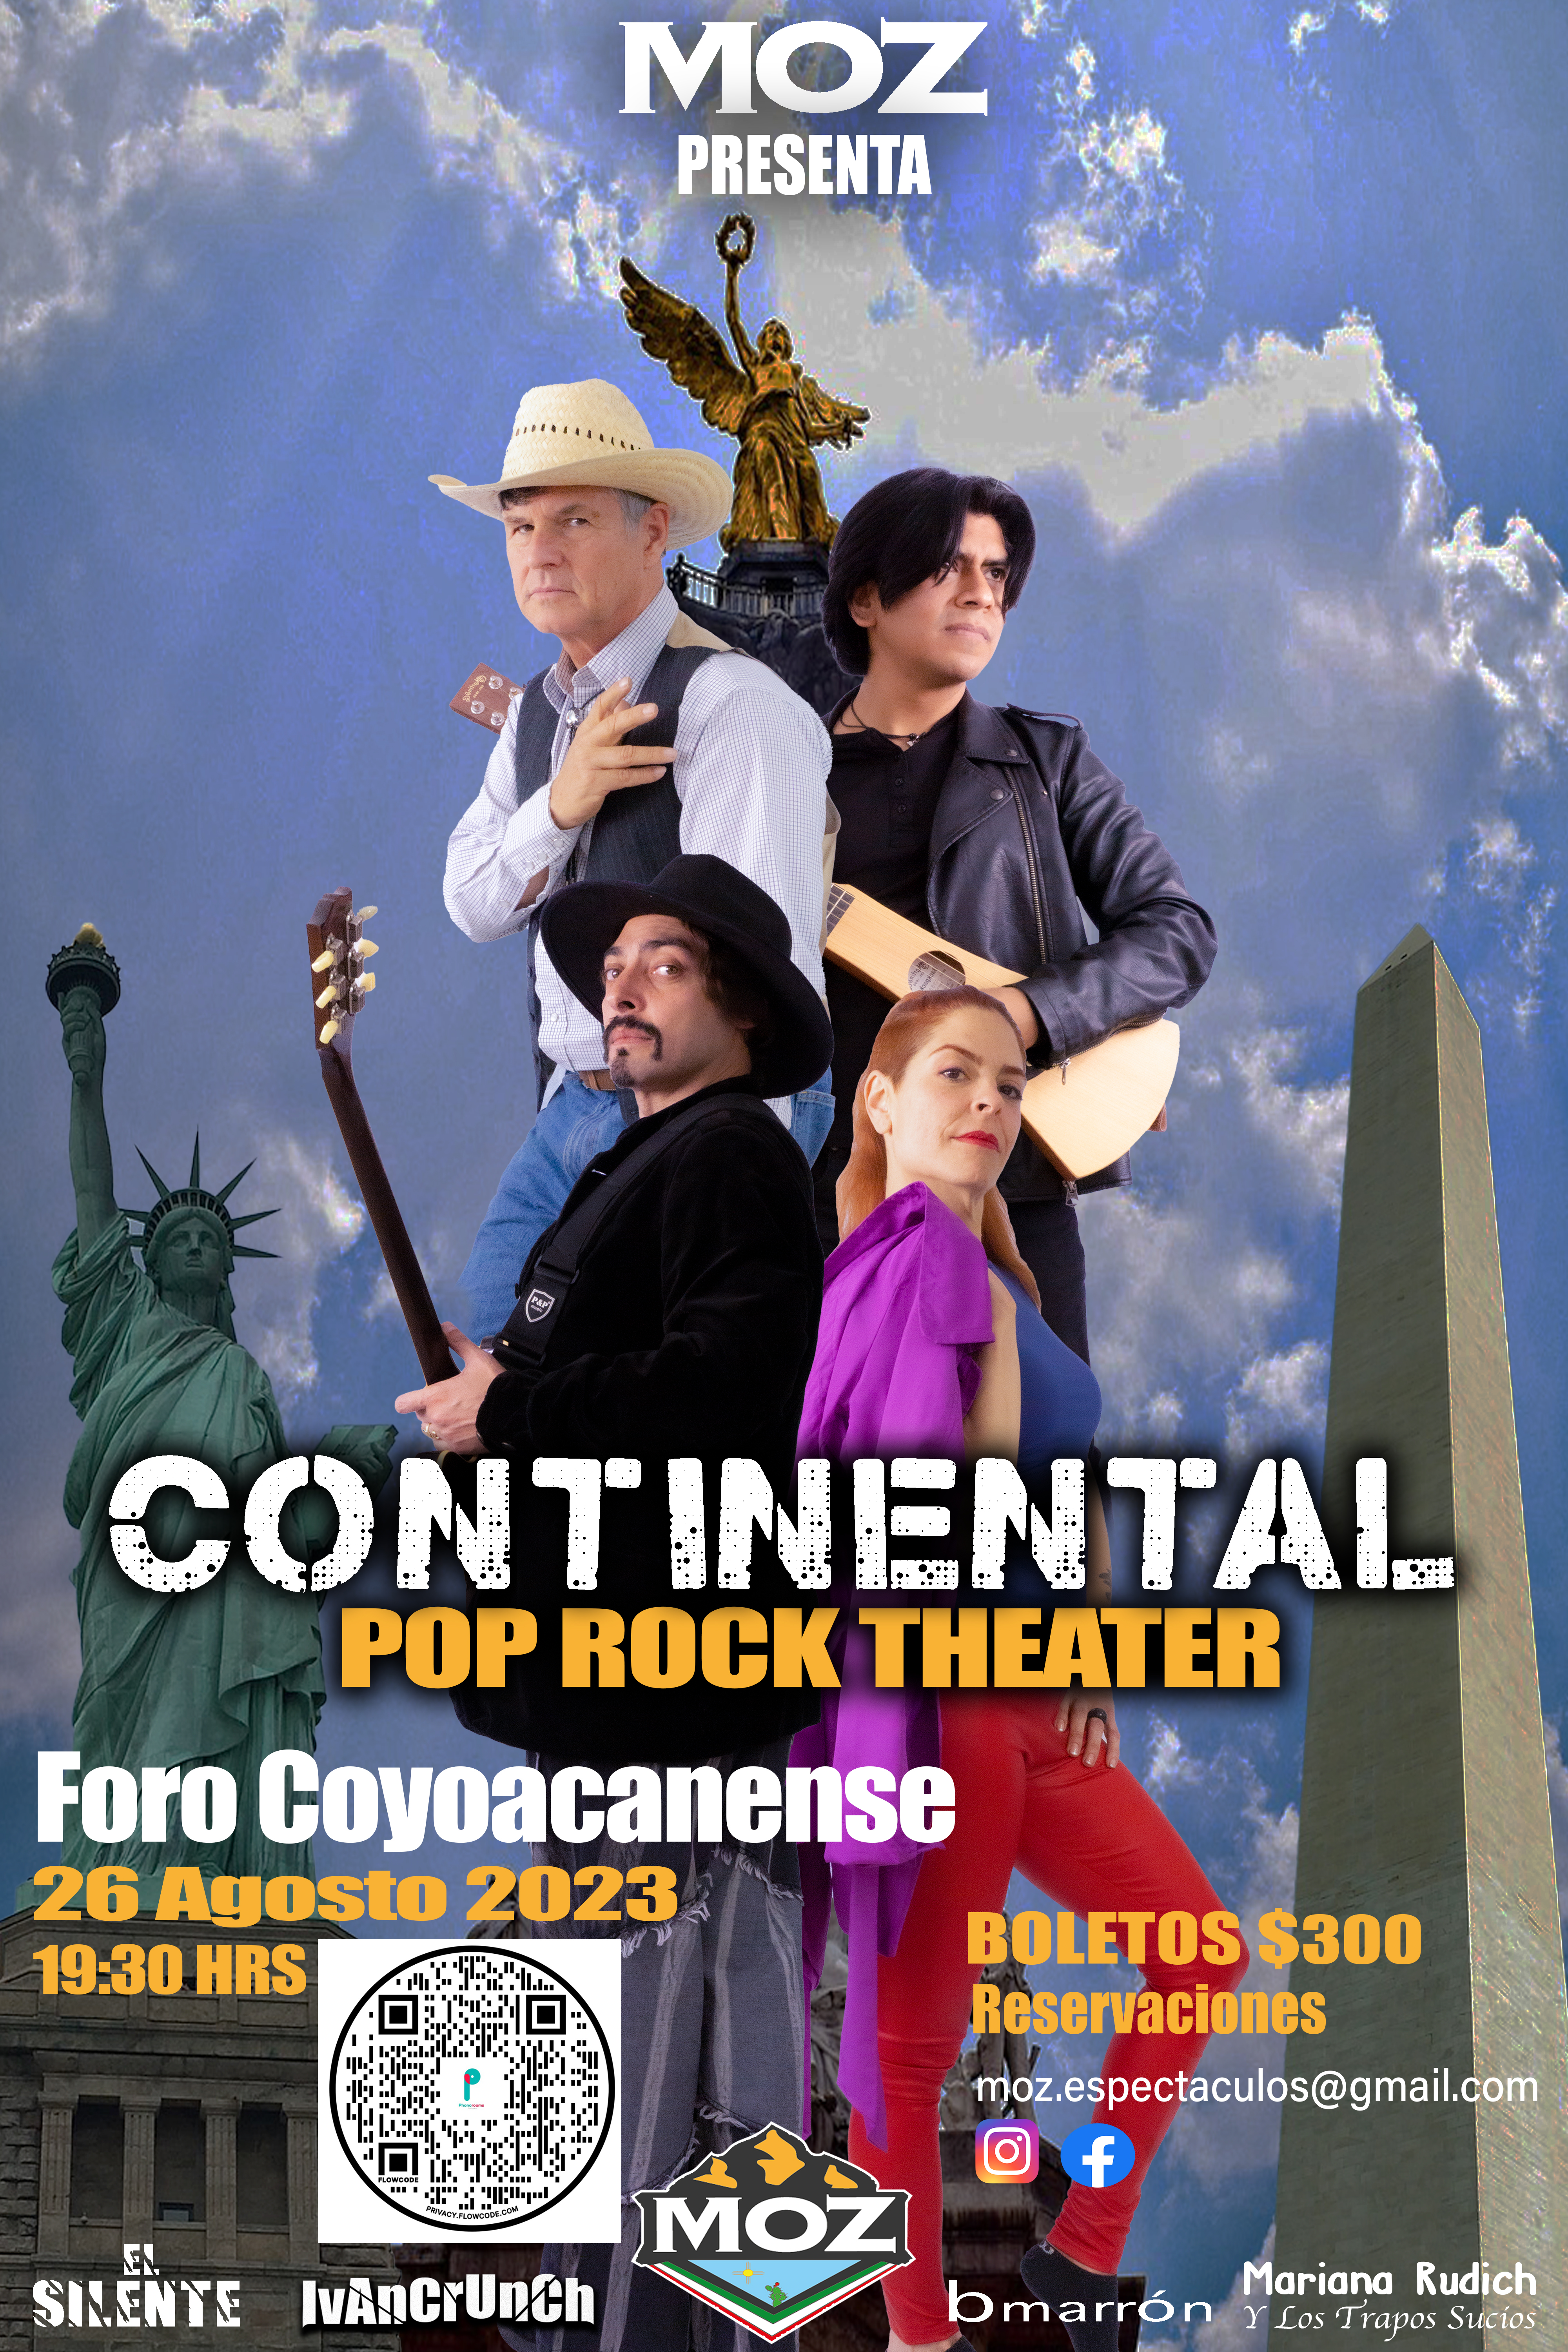
\includegraphics[scale=0.03]{graphics/MOZ_CartelFinal.jpg}};  
 \end{tikzpicture}
 
 %% Pic 6
 \begin{tikzpicture}[overlay]
  \node[anchor=south west] at (13,-7.5) {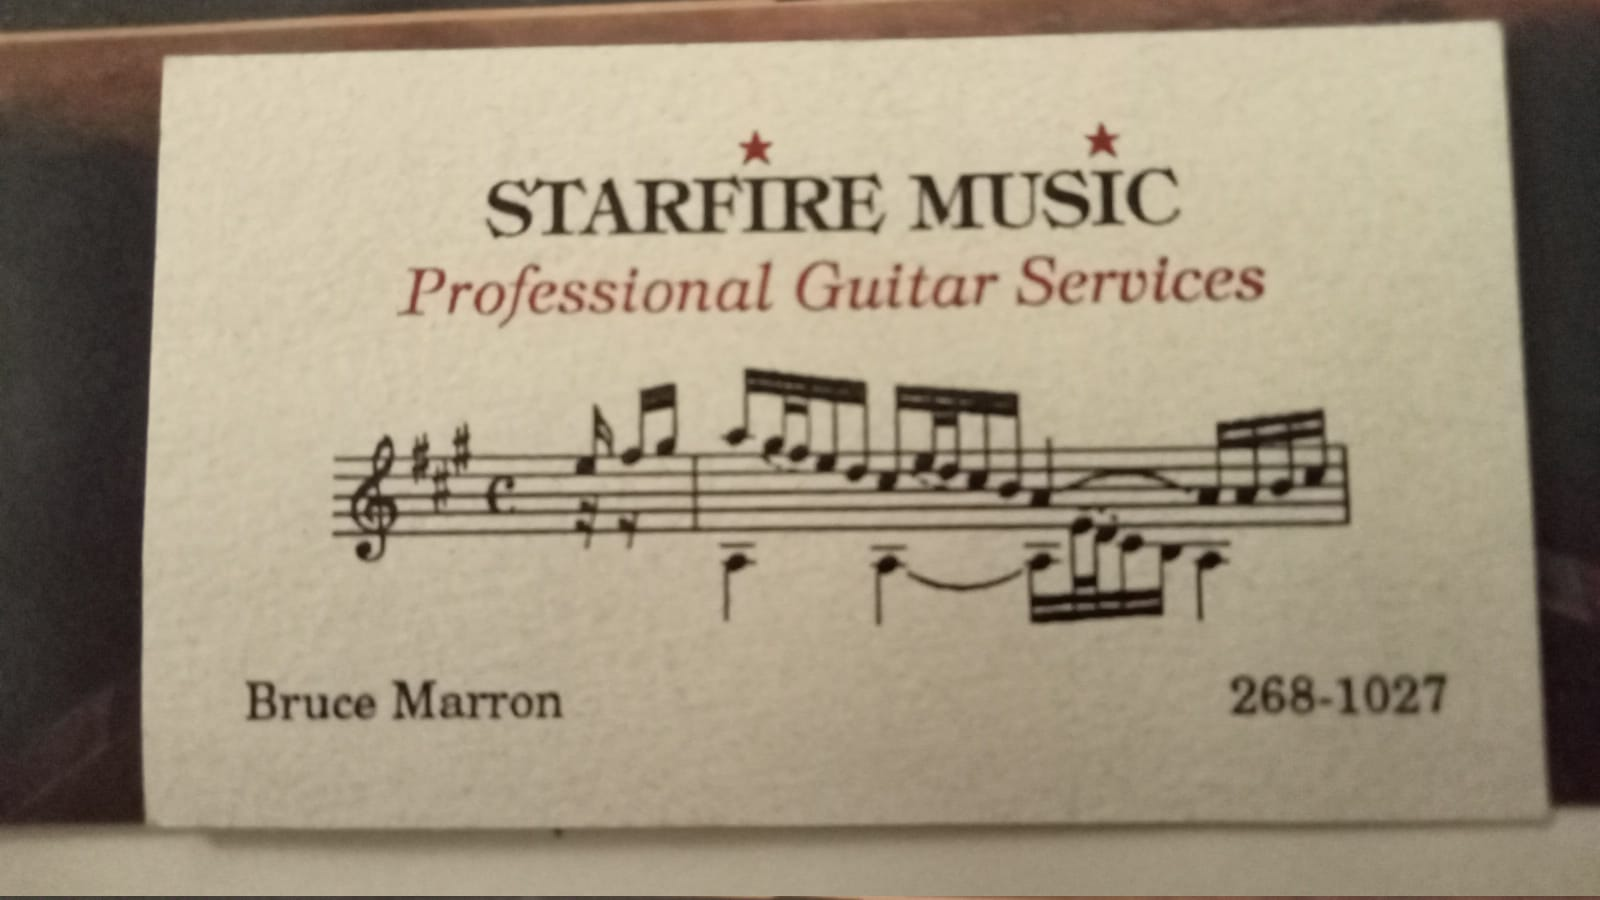
\includegraphics[scale=0.11]{graphics/Marron_StarfireMusic.jpeg}};  
 \end{tikzpicture}
 
 
 


\end{resume}
\end{document}







